%!TeX root=../../master.tex
\section{Gesture Recognition}\label{sec:gesturerecognition}
The system lets users control smart devices in their home by performing certain gestures.

Gesture recognition can generally be split into two categories: 
Camera-based and motion-based \cite{Kela2006}. 
Examples of camera-based gesture recognition systems are the ``Gesture Pendant'' \cite{starner2000gesture} and the Kinect \cite{kinect}, 
and an example of a motion-based system is the Reemo \cite{Reemo}.

The camera-based solution require that the limbs, 
used to perform gestures, 
are visible to the camera, 
and as such \emph{static} cameras placed in a room, 
may be rendered useless if the user turns his back against them. 
In addition, furniture and other people may stand in between them, 
and obstruct the line of sight between the camera and the user.
This would likely not happen with the ``Gesture Pendant'',
because it is worn by the user, 
but the user would have to make sure that the pendant is always outside of any clothes worn.
Putting on a sweater or wrapping yourself in a blanket, 
might block the view of the camera.

Motion-based solutions can employ various different sensors on the person,
such as accelerometers and gyroscopes, 
and depending on the type of sensor, 
different methods can be used to recognize gestures.
As mentioned in \Cref{sec:wearables}, accelerometers are present in about half of the wearables. 
Because of this, we will focus on finding a solution using accelerometer, 
so that we do not have to use additional hardware, such as cameras. 

In the following section, we will describe a gesture recognition system called the \$3 Gesture Recognizer. 

\subsection{\$3 Gesture Recognizer}\label{sec:threedollar}
The \$3 Gesture Recognizer is a gesture recognition system, 
created by Sven Kratz and Michael Rohs, 
and is presented in the paper ``A \$3 Gesture Recognizer – Simple Gesture Recognition for Devices Equipped with 3D Acceleration Sensors'' \cite{threedollar}.

The system is based on the \$1 Recognizer by Wobbrock \etal \cite{wobbrock2007gestures}, 
and adds the ability to detect \emph{three dimensional gestures}, 
rather than being limited to two dimensional gestures from the \$1 Recognizer.

Both of these systems are designed to be easy to use by anyone for fast prototyping of user interfaces, 
which makes them appropriate for use in this project.
The \$3 Gesture Recognizer, however, is better suited, 
as it is capable of recognizing more gestures because it utilizes three dimensional data.
This means that users have even more options for personalizing the gestures, 
that they will use to control their home with.

The \$3 Gesture Recognizer requires the user to train a gesture about five times, 
before it can deliver adequate recognition rates. 
This provides a good experience for the user, 
as he does not need to spend much time training the system before he is able to use it.
Whenever a user trains a gesture, 
a new gesture trace is stored and associated with a gesture class. 
A gesture class that has been trained five times, 
has five gesture traces stored.

The \$3 Gesture Recognizer works by sampling a three-axis accelerometer, 
and subtracting the current acceleration from the previous acceleration, 
to acquire an acceleration delta.
These acceleration deltas are then used to create a three dimensional time series, 
called gesture trace $T$.
This is illustrated in \Cref{fig:onedollar-gesturetrace}. 
Note that this illustration only shows two-dimensionsional traces, 
as the illustration is from Wobbrock \etal \cite{wobbrock2007gestures}.
The gesture traces in \cite{threedollar} are three-dimensional. 

\begin{figure}[!htb]
	\centering
	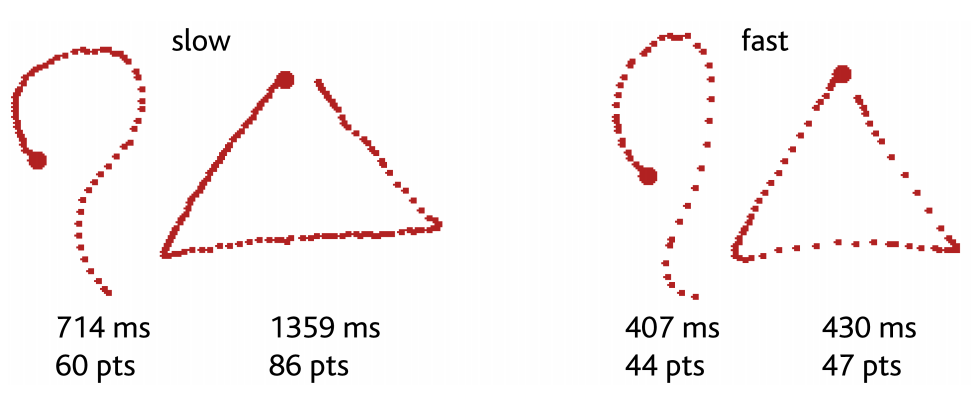
\includegraphics[width=0.8\textwidth]{images/1-dollar-gesturetrace.png}
	\caption{A slow and fast question mark and a triangle, made by subjects using a stylus on a Pocket PC. Note the considerable time differences and resulting numbers of points. Image and text is from Figure 3 in \protect\cite{wobbrock2007gestures}.}
	\label{fig:onedollar-gesturetrace}
\end{figure}

\Cref{fig:onedollar-gesturetrace} also shows that the gesture traces can contain a different number of points, 
when performing the same gesture at different speeds.
Because of this, the \$3 Gesture Recognizer \emph{resamples} $T$, 
so that it contains a fixed number of points. 
In \cite{threedollar}, the number of points $N$ is \num{150}, 
with equal distance between the points.
If $N$ is set to a lower value, then precision is lost. 
If $N$ is set to a higher value, then computational cost increases.
After resampling the points, 
$T$ is rotated in an attempt to correct for any rotational error, 
and finally it is scaled to fit inside of a cube of $100^3$ units, 
to compensate for the fact that users may perform inconsistently sized gestures.


Once all of these transformations have been performed, 
the gesture trace is matched against all the trained gestures. 

The gesture traces are stored as matrices with three columns, 
one for each axis of the accelerometer, 
where each row represents an acceleration delta.
These matrices are compared by calculating the distance between them using, 
the average mean square error (MSE).
The distance is then converted to a score in the range $[0,1]$, 
using an equation by Wobbrock \etal, 
modified to work with three-dimensional traces.
The scoring equation from \cite{threedollar} is shown in \Cref{eq:gesture-scoring}:
\begin{equation}\label{eq:gesture-scoring}
    score = 1-\frac{d}{0.5\sqrt{3l^2}}
\end{equation}

A scoring table is then created, 
listing all of the trained gesture traces and their score. 
The table is sorted by the highest score.
To reduce the number of false positives, 
the following scoring heuristic is used \cite{threedollar}:

\begin{enumerate}
	\item {$\epsilon$ is defined as the threshold score.}
	\item {Iff the highest-scoring candidate in the score table has a score $> 1.1\epsilon$, return this candidate’s gesture ID.}
	\item {Iff, within the top three candidates in the score table, two candidates exist of the same gesture class and have a score > 0.95$\epsilon$, respectively, return the gesture ID of these two candidates.}
	\item {Else, return ``Gesture not recognized!''.}
\end{enumerate}

%%% Local Variables:
%%% mode: latex
%%% TeX-master: "../../master"
%%% TeX-command-extra-options: "-shell-escape"
%%% End:
